\subsection{Anforderungsspezifikation}

\subsubsection{Funktionale Anforderungen}

\paragraph{Brief Use-Cases}

Im Folgenden ist das Use-Case-Diagramm dargestellt.
\begin{figure}[h]
	\centering
	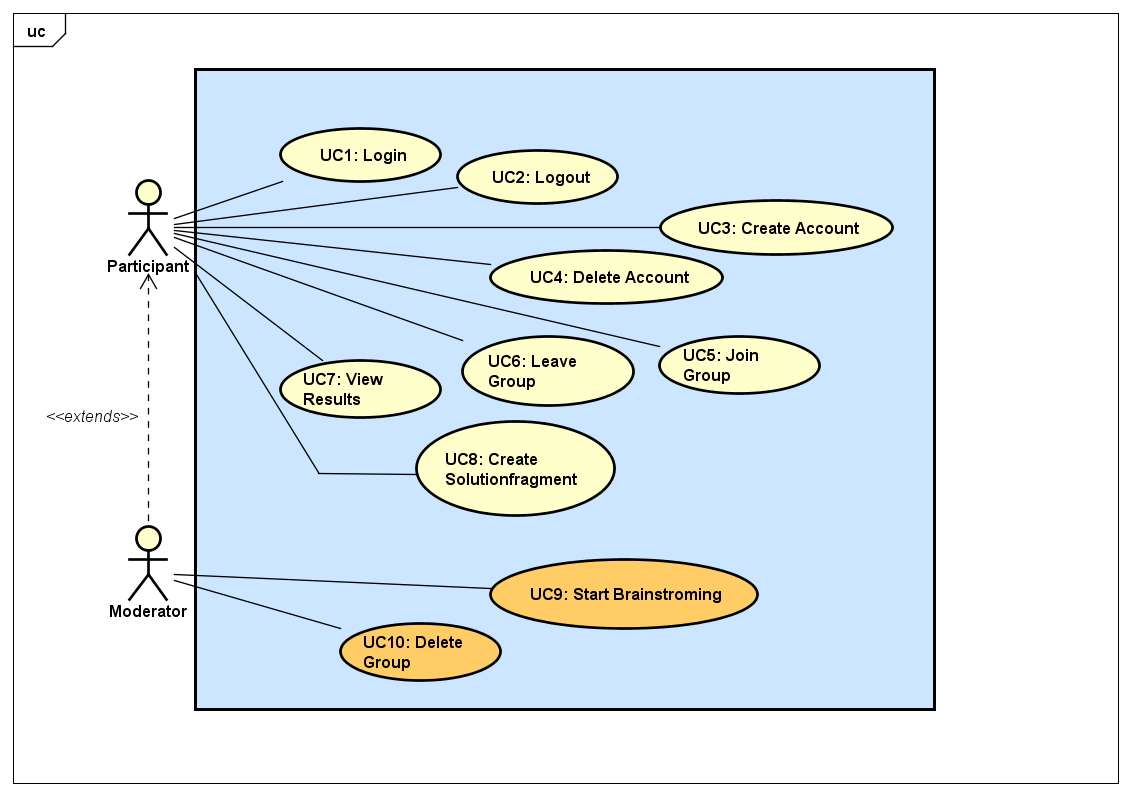
\includegraphics[width=1\linewidth]{img/anforderungen/UC-Methode635}
	\caption{Use-Case-Diagramm}
	\label{fig:ucmethode-635}
\end{figure}

Jeder Use-Case hat den nachfolgend kurz (\textit{briefly}) beschriebenen  Funktionsumfang. Die Hauptaktivitäten UC7-9 sind am Schluss \textit{fully-dressed} beschrieben.

\begin{basedescript}{%
		\desclabelstyle{\multilinelabel}
		\desclabelwidth{4.5cm}}
	\item[\textit{UC1: }Login] Als Participant möchte ich mich mit Benutzernamen und Passwort in das System einloggen können.
	\item[\textit{UC2: }Logout] Als eingeloggter Participant will ich mich ausloggen, sodass das Startfenster wieder erscheint.
	\item[\textit{UC3: }Create Account] Als Benutzer der Applikation möchte ich mich registrieren können.
	\item[\textit{UC4: }Delete Account] Als Benutzer will ich meinen erstellten Account wieder löschen können.
	\item[\textit{UC5: }Join Group] Als Participant will ich einer bereits existierenden Gruppe beitreten können.
	\item[\textit{UC6: }Leave Group] Als Participant will eine beigetretene Gruppe verlassen können.
	\item[\textit{UC7: }View Results] Als Participant will ich, nachdem eine Brainstorming Session durchgeführt wurde, das Resultat meiner Gruppe einsehen können.
	\item[\textit{UC8: }Create\\Solutionfragment] Als Participant will ich während einer Brainstorming Session ein Lösungsfragment erstellen und einreichen können. 
	\item[\textit{UC9: }Start \\Brainstorming] Als Moderator will ich eine Brainstorming Session starten.
	\item[\textit{UC10: }Create Group] Als Moderator will ich eine Gruppe erstellen können. 
	\item[\textit{UC11: }Delete Group] Als Moderator will ich eine Gruppe löschen können.
\end{basedescript}

\paragraph{Fully-Dressed Use-Cases}


\paragraph{Abuse-Cases}
%Abuse cases?
Um einem Missbrauch der Applikation entgegenzuwirken, sind neben den Use-Cases auch Abuse-Cases definiert. Diese helfen, mit unangebrachtem Inhalt und unangebrachter Verwendung umzugehen.
\begin{basedescript}{%
		\desclabelstyle{\multilinelabel}
		\desclabelwidth{4.5cm}}
	\item[\textit{AC1: }Unangebrachte Lösungsfragmente] Ein Participant könnte unangebrachte Inhalte in einer Gruppe hinzufügen. Um dies zu verhindern, könnte eine die Applikation um eine Funktion erweitert werden, die es dem Moderator erlaubt, Benutzer auszuschliessen.
\end{basedescript}

%Sequence diagram
\paragraph{Sequenzdiagramm}
Der Ablauf der Kernlogik ist der Abbildung \ref{fig:seq-methode635} zu entnehmen. Darin ist der Prozess vom Erstellen der Gruppe (UC10) bis zum Abschliessen der Brainstorming Session modelliert.
\begin{figure}[h]
	\centering
	\makebox[\textwidth][c]{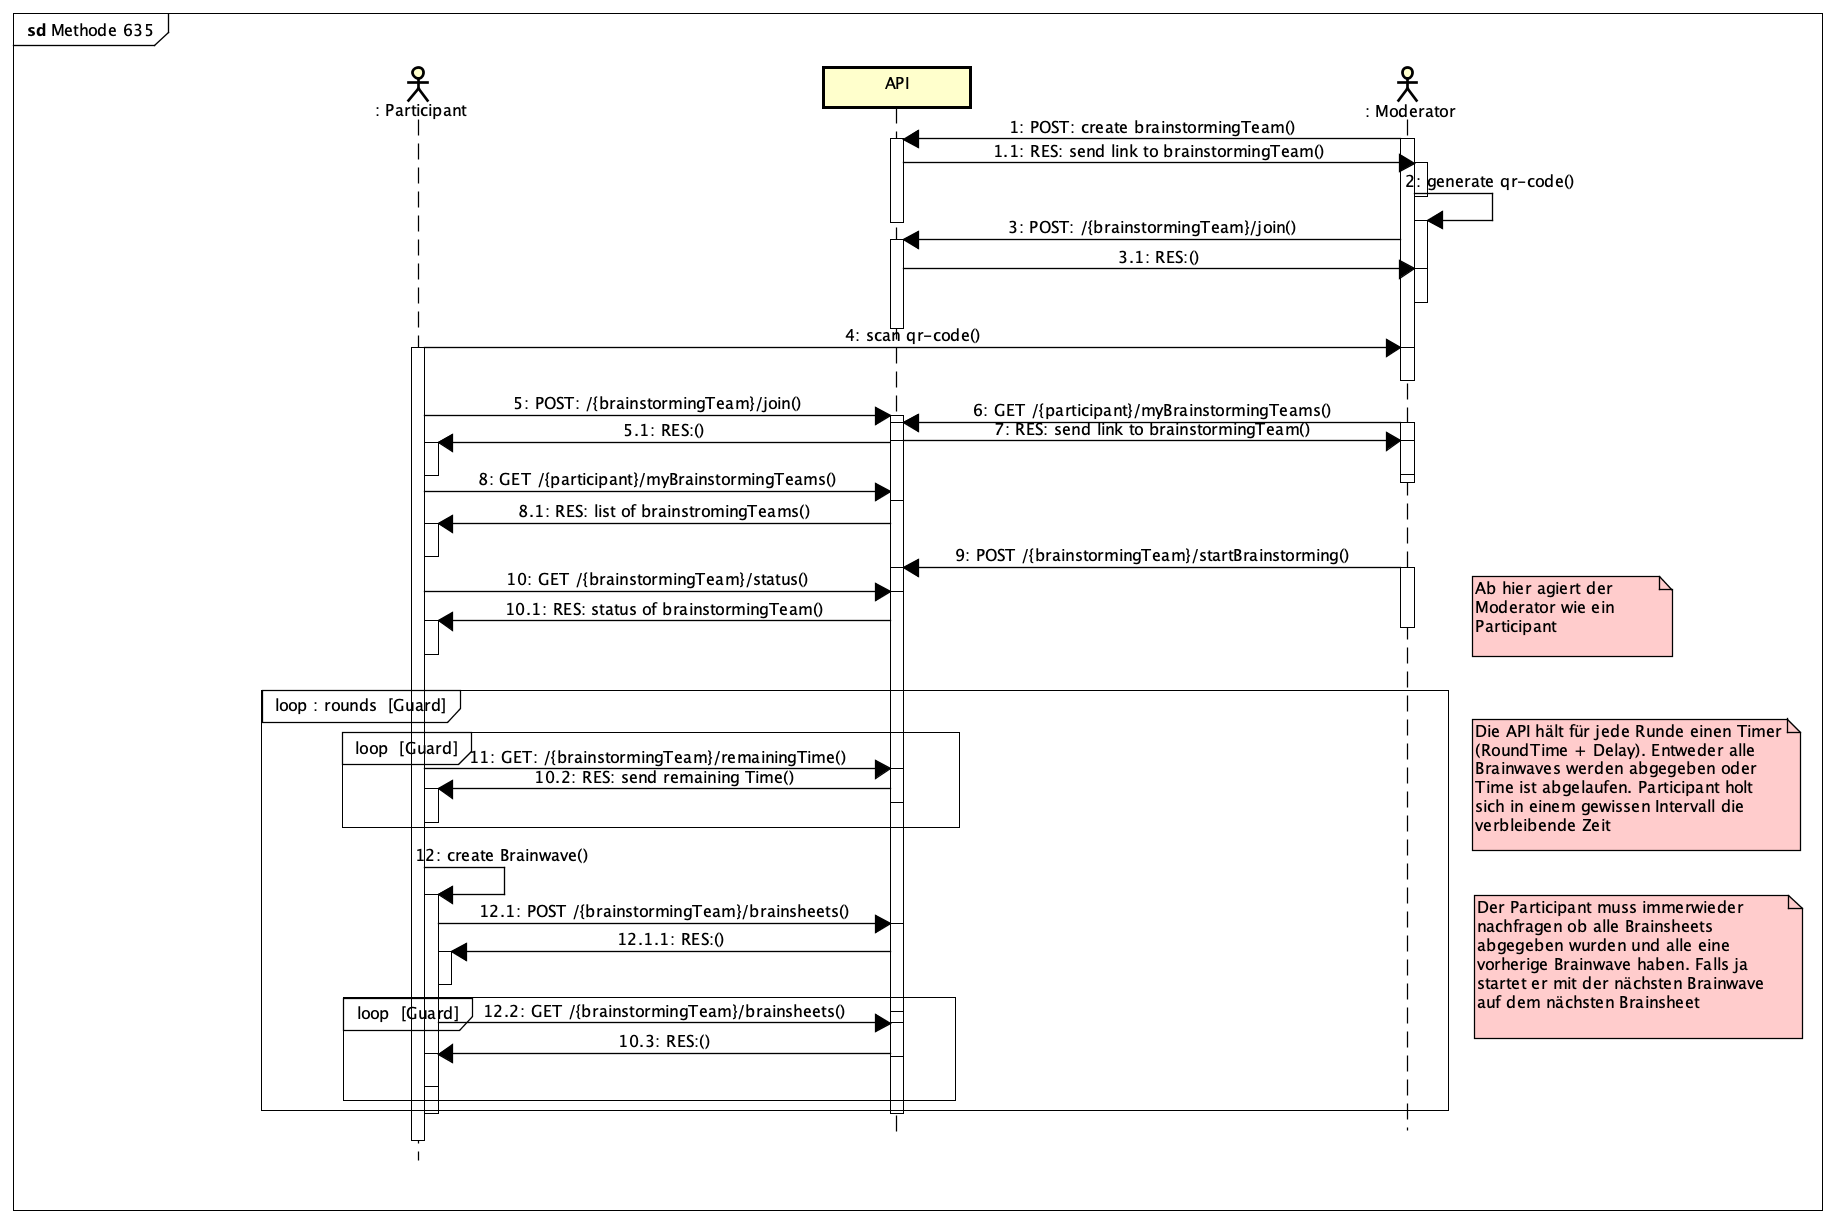
\includegraphics[width=1.2\linewidth]{img/anforderungen/Seq-Methode635}}
	\caption{Sequenzdiagramm}
	\label{fig:seq-methode635}
\end{figure}


\subsubsection{Nicht-Funktionale Anforderungen}
Beim Thema Nicht-Funktionale Anforderungen halten wir uns an die Standards ISO 9126\cite{ISO9126} bzw. dessen Nachfolger ISO 25010\cite{ISO9126_ISO25010}. Beide ISO-Normen sind sich sehr ähnlich und liefern eine gute Checkliste für jegliche Art von Systemanforderungen.

\begin{figure}[h]
	\centering
	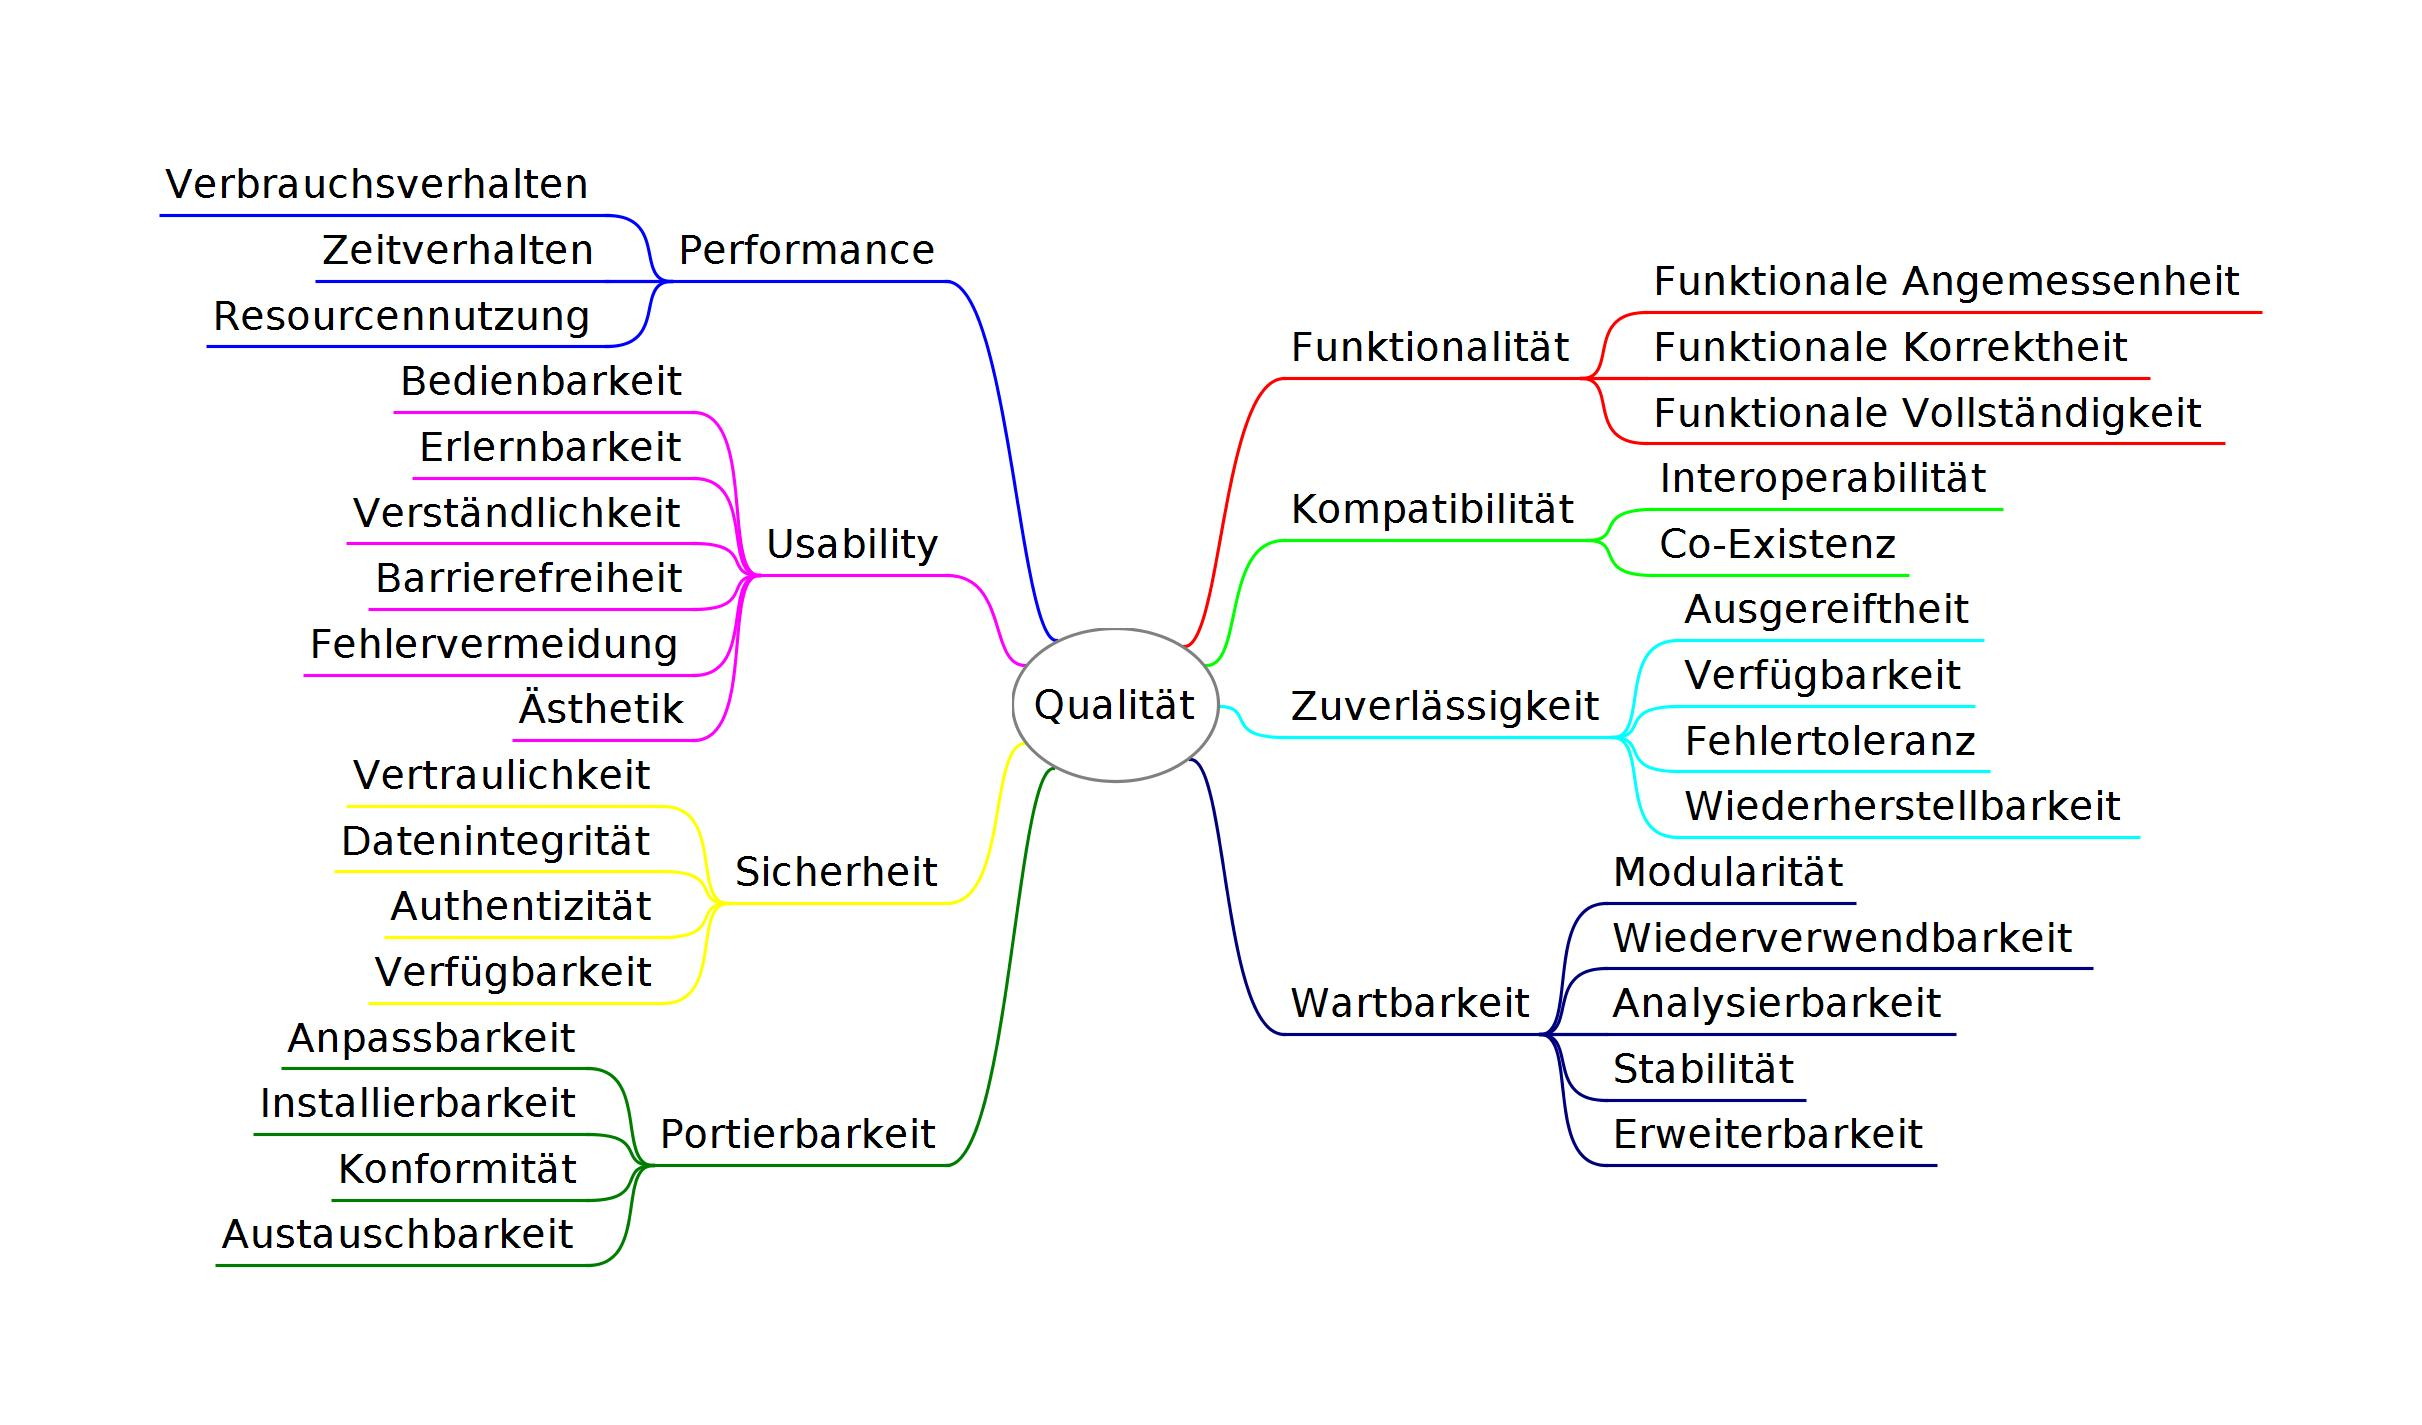
\includegraphics[width=1\linewidth]{img/anforderungen/quality}
	\caption[Anforderungskategorien nach ISO 25010]{Anforderungskategorien nach  ISO 25010}
	\label{fig:ISO 25010}
\end{figure}

%TODO Bild Link: https://blog.seibert-media.net/blog/2018/05/14/qualitaet-funktionale-und-nichtfunktionale-anforderungen-in-der-software-entwicklung/

Diese Normen sind sehr umfangreich gestaltet. Wir werden uns daher auf die, für uns, wichtigsten Anforderungen konzentrieren. Um genaue und erfüllbare nicht-funktionale Anforderungen zu definieren, müssen die SMART-Kriterien \cite{SMART} erfüllt sein. 

\begin{description}[leftmargin=!,labelwidth=\widthof{\bfseries Wiederverwendbarkeit}]
	\item[Ressourcennutzung] Die internen Ressourcen Kamera, Dateisystem dürfen nur bei effektivem Bedarf benützt werden. Die CPU-Ressourcen\-nutzung darf im Durchschnitt pro Minute maximal zu 40\% in Anspruch genommen werden.\footnote{Referenzsystem Android: Huawei P10 mit Android Version 8.0.0 mit Hisilicon Kirin 960 CPU und 4GB RAM}\footnote{Referenzsystem iOS: iPhone 6 mit iOS Version 12 mit Dual-core 1.4 GHz Typhoon CPU und 1GB RAM}
	
	\item[Bedienbarkeit] Wenn eine Aktion länger als 1-2s geht, soll dem User ein Wartesymbol angezeigt werden. 
	
	\item[Ästhetik] Die Benutzeroberflächen der Applikation sind so gestaltet, dass die Elemente wiedererkennbar sind (Buttons haben gleichen Stil, leere Textfelder haben Platzhalter). 
	
	\item[Vertraulichkeit] Die Daten einer Brainstorming Session können nur von der zugehörigen Gruppe eingesehen werden. 
	
	\item[Anpassbarkeit] Die Anpassung bestehender oder Integration neuer Brain\-storming-Methoden muss gewährleistet sein.
	
	\item[Installierbarkeit] Die Installation der Applikation auf einem Endgerät erfolgt durch das Ausführen eines *.apk oder *.app. Dieser Prozess soll unter 1 Minute geschehen.
	
	\item[Co-Existenz] Sollte zu einem späteren Zeitpunkt entschieden werden ein Web-Frontend zu programmieren, muss dieses co-existent mit der Xamarin Applikation existieren können.
	
	\item[Wiederherstellbarkeit] Im Falle eines fehlerhaften Features, muss es innerhalb eines Werktages möglich sein, die Applikation wieder auf den letzten funktionierenden Stand zurück zu holen und erneut zu deployen.	
	
	\item[Wiederverwendbarkeit] Die Auswertung von 'Duplicated Code' in SonarQube soll unter 8\% liegen. Dies deutet auf eine hohe Wiederverwendbarkeit hin, denn ansonsten müsste der Code kopiert werden. 
	
	%TODO: Referenz auf Use Cases
	\item[Analysierbarkeit] Das Ausführen eines Use-Cases muss durch Analyse von Logfiles erkennbar sein.
\end{description}
